Well, this bodes ill.~Quoting \texttt{@foone@digipres.club} at
\url{https://digipres.club/@foone/109736253785929072}

\begin{figure}
\centering
\pandocbounded{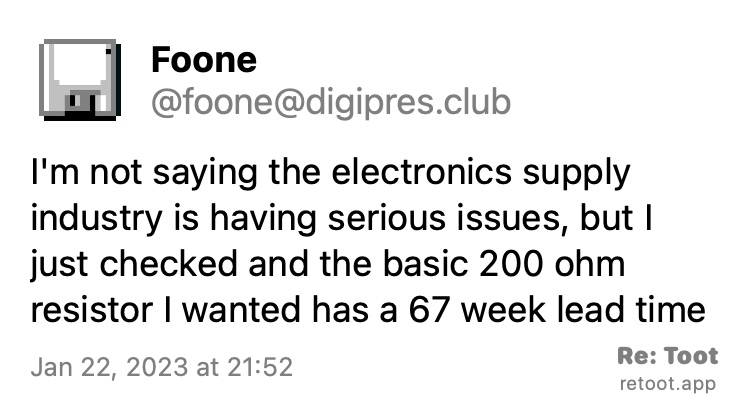
\includegraphics[keepaspectratio]{\%7B\%7Bsite.url\%7D\%7D/img/long-lead-resistor.jpg}}
\caption{Post by Foone. ``I'm not saying the electronics supply industry
is having serious issues, but I just checked and the basic 200 ohm
resistor I wanted has a 67 week lead time'' Posted on Jan 22, 2023 at
21:52. https://digipres.club/@foone/109736253785929072}
\end{figure}

Our economy is in a pretty precarious state. If basic resistors like
\emph{that} have that long of a lead time I think it can be safely said
that we're on the precipice of dire straits. Once upon a time we used to
sell those sorts of things as rather plentiful basics at RadioShack when
I was in consumer electronics retail.

We won't have to worry about ``virtual reality'' or the ``metaverse'' at
the rate things are deteriorating either. Quoting
\texttt{@twitnews@twit.social} at
\url{https://twit.social/@twitnews/109730924729178428}

\begin{figure}
\centering
\pandocbounded{
\includegraphics[keepaspectratio]{\%7B\%7Bsite.url\%7D\%7D/img/goodbye-hololens.jpg}}
\caption{Post by TWiT News Feed. ``Microsoft has laid off entire teams
behind Virtual, Mixed Reality, and HoloLens Windows Central -
windowscentral.com/microsoft/m\ldots{} In addition to the death of
AltSpaceVR, Microsoft has also culled the entire team behind the popular
MRTK framework. MRTK is Microsoft's''Mixed Reality Took Kit,'' which is
a cross-platform framework for spatial anchors in virtual reality
spaces. MRTK was built for Unity VR integrations, and works with Meta's
headsets with a focus on HoloLens.'' Posted on Jan 21, 2023 at 23:17 at
https://twit.social/@twitnews/109730924729178428}
\end{figure}

The tech sector has taken a pounding as we've tried to come out of the
acute phase of the COVID-19 pandemic. The tech sector \emph{had} a
pretty bright future. The backlash from the MAGA cult found a pretty
vulnerable target in the tech sector as it appeared to be a cause of
many evils. After all, it enabled the lockdowns and the altered ways of
living that got the cult so very upset. Since it enabled those things
the cult is doing what it can to punish big tech.

The problem lurking in the corner that overshadows the rest of this is
the debt ceiling. The Republican Party's majority in the House is very
small. Only four votes can be lost in a vote for the Republicans to
still prevail if every member of the House participates in the vote.
Only one member of the Republican caucus voted in favor of the last debt
ceiling increase way back in \emph{December 2021} and unfortunately he
no longer serves in Congress. It is hard at the moment to nail down how
many are ready to vote no regardless of what they are presented with.

This is the ``Thelma and Louise'' year, I guess.
